%%%%%%%%%%%%%%%%%%%
% Related Work
%%%%%%%%%%%%%%%%%%%
\section{Related Work and Background}
\label{sec:related}
%
This section reviews other systems that provide memory protection.
%
The systems are broadly classified based on their application
domains.
%
We focus first on sensor networks and then survey the more general
space of desktop and server computing systems.
%
We conclude this section with a brief overview of SOS operating system.
%
%=====================================================================
\subsection{Sensor Networks}
%
As sensor networks are envisioned for long-term deployments, several
projects have addressed reliability as a primary design
concern~\cite{tkernel06sensys,regehr06utos,dutta05ipsn}.
%-------------------------------------------------------------
\subsubsection{Naturalization --- \emph{t-kernel}}
%
\emph{t-kernel}~\cite{tkernel06sensys}, a runtime for Mica motes, also
rewrites binaries to make them safe for execution.
%
Harbor and \emph{t-kernel} represent different points in the design space of
software-based protection mechanisms.
%
\emph{t-kernel} enforces a strong isolation boundary between the application and
the kernel.
%
Through a process called \emph{naturalization}, the application binary is
rewritten on the sensor node to guarantee that the \emph{t-kernel} can
always safely regain control of the processor, even, for example, in the
presence of application infinite loops that could otherwise hang the
system.
%
The rewritten application binary contains an entire TinyOS operating system
image, in contrast to Harbor, where multiple modules within an
application are prevented from corrupting one another.
%


\emph{t-kernel} also implements software-based differentiated
virtual memory,
%
which translates the addresses for all memory accesses made by a program
into the heap segment.
%
The overhead of virtual memory is unpredictable and can be very
high in the event of a swap from external flash.
%
Harbor does not implement virtual memory, but does enforce memory isolation at a
finer granularity than \emph{t-kernel}.
%
In particular, Harbor can protect application modules from
one another.
%

Harbor does not address control flow isolation, except as required to
enforce memory isolation; in particular, it cannot force a buggy module
stuck in an infinite loop to relinquish control of the CPU.
%
\emph{t-kernel} requires external flash memory, whereas Harbor makes use of
on-chip flash memory only.
%
%-------------------------------------------------------------
\subsubsection{Safe OS Extensions --- UTOS}
%
Safe TinyOS~\cite{regehr06utos} uses CCured~\cite{ccured02necula} and static
analysis techniques to provide memory safety for TinyOS applications.
%
CCured performs complex pointer analysis to mark pointers as safe or
unsafe.
%
Much driver code performs arbitrary typecasts that can cause CCured to
fail or conservatively mark pointers as unsafe, which introduces a
performance penalty as the CCured run-time performs bounds checks on
unsafe pointers during code execution.
%
CCured provides memory safety at a much finer granularity than Harbor.
%

The UTOS framework allows untrusted extensions to
safely interface with Safe TinyOS components.
%
UTOS extensions are made type-safe and memory-safe using CCured and a
backend service that copies buffers when they are exchanged between the
extension and the Safe TinyOS core.
%
Extensions are not allowed to interact with one another.
%
Harbor allows safe buffer transfers without copying, and allows extensions
to interact, but its current simple runtime check infrastructure introduces
overhead that CCured can sometimes avoid.
%

The UTOS backend service also mediates resource requests and prevents any
extension from starving other extensions in the system.
%
Harbor does not make any guarantees on fair resource allocation.
%
%-----------------------------------------------------------------
\subsubsection{Application Specific Virtual Machines --- Mat\'e}
%
Application Specific Virtual Machines (ASVM) such as
Mat\'e~\cite{asvm05nsdi}~\cite{levis02mate} and
Agilla~\cite{agilla05ipsn} are domain specific interpreters that
execute high-level application scripts.
%
Both Harbor and ASVMs provide memory safety to applications, albeit
through different mechanisms.
%
Harbor isolates applications from one another.
%
ASVM performs type and bounds checks on all memory accesses.
%
ASVM's checks are in some ways more stringent than Harbor's protection,
since the type safety of the instruction set also prevent scripts from
corrupting \emph{their own} memory.
%
However, errors in ASVM's native code implementation might corrupt any
memory on the node.
%
Further, for efficiency, ASVMs are designed to be easily extensible to
customize the interpreters for a specific application domain.
%
The extensions can also be introduced dynamically~\cite{balani06dvm}.
%
The ASVM extensions implement powerful high level opcodes that perform
complex operations.
%
The extensions are implemented in non-type safe languages and can be
buggy.
%
ASVMs could thus use Harbor's isolation to become more robust to errors in
extensions.


The trade-offs between ASVMs and Harbor are evaluated in detail in
Section~\ref{sec:eval}.
%
Harbor has a significantly lower execution overhead compared than ASVM,
%
but its run-time checks 
%introduced by Harbor 
increase code size.
%
%-----------------------------------------------------------------
\subsubsection{Type Safe Languages --- Virgil}
%
Type-safe languages provide memory safety at a fine granularity.
%
Type-safe languages for resource constrained microcontrollers is an
emerging area of research.
%
Most of the software developed for embedded systems is written in
unsafe languages such as C (or even assembly for low-level drivers). 
%
The popular sensor network programming language NesC~\cite{gay03nesc}
contains minimal extensions to C (such as the \texttt{atomic} keyword)
to prevent race conditions.
%
However, it does not address memory safety.


A common criticism of safe languages or unsafe languages retrofitted
with type information~\cite{ccured02necula} is their excessive CPU and
memory consumption.
%
This often makes them unsuitable for resource constrained sensor
nodes.
%
Virgil~\cite{titzer06virgil} is a new programming language that
attempts to address some of these concerns.
%
By explicitly separating initialization time from run time, Virgil
allows an application to build complex data structures during
compilation and then run directly on bare hardware without a virtual
machine or a language run time.
%
The separation allows the entire program heap to be available at
compile time and enables new optimizations that reduce memory size.
%
Virgil does not support dynamic memory allocation.
%
Therefore, it is currently suited for building application specific
static operating system images such as TinyOS~\cite{levis05t2}.
%
An interesting area of future research is to explore safe languages
(such as Virgil) as a primary extensibility mechanism for dynamic
sensor operating systems such as SOS~\cite{ram05sos}.
%
SPIN project~\cite{spin95sosp} at University of Washington explored
safe languages as the primiary extensibility mechanism in desktop
operating systems.

Finally, a safe language restricts an implementation to a single
language; it ignores a large base of existing code.
%
Harbor operates on compiled binaries and is therefore independent of
any programming language and is applicable to all existing code.
%
Type safe languages require unsafe extensions to interface to
low-level hardware\footnote{Virgil extends type safety to the
  hardware}, though these extensions could be used sparingly.
%
Another problem with type-safe languages is the size of the system
that needs to be trusted.
%
A complete language compiler and run-time consists of an optimizer
that uses complex analysis to improve run-time efficiency.
%
This is a large and complicated code base, all of which needs to be
trusted.
%
In contrast, for Harbor, only the run-time components and the simple
verifier needs to be trusted.
%
The size of this system is considerably smaller than the size of a
compiler.
%
% VM*~\cite{vmstar05sensys} is a virtual machine construction kit
% targets resource constrained sensor nodes and supports a subset of the
% JAVA programming language.
% %
% The VM* framework automatically generates an application specific
% virtual machine.
% %
% The virtual machine is optimized to include only parts of the
% interpreter and the run-time that are needed.
% %
% A native API exposes the OS and hardware services to the JAVA
% applications.
% %
% VM* addresses the development of applications in JAVA but the
% underlying operating system and device drivers are still written in
% non type-safe languages such as C or assembly.
% %
% JAVA applications in VM* are type-safe.
% %
% Unlike Harbor and UTOS, the VM* applications are not isolated from the
% operating system.
%
%Sympathy, a debugging framework, has focussed on developing
%network-level protocols to diagnose/localize
%problems~\cite{nithya05sympathy} 
%
%We can leverage Sympathy framework to send diagnostic information to
%the basestation whenever an exception is triggered in Harbor
%
%At present, hardware support in sensor nodes to achieve high
%dependability is absent, with reboot of the entire node being the
%most common approach~\cite{dutta05ipsn}.
%
%

Recently, RETOS operating system~\cite{retos07spots}, also provides
memory protection for applications through a rewrite of compiled binary.

%=========================================================================
\subsection{Software-based Techniques}
%
The design considerations for an embedded sensor system are vastly
different from a desktop/server system.
%
Still, some of the features in Harbor have been motivated from the
large range of software-based memory protection techniques proposed
for desktop/server systems.
%
%------------------------------------------------------------
\subsubsection{Software-based Fault Isolation (SFI)}
%
Software-based Fault Isolation (SFI) is a general technique that
restricts the address range of stores, jumps and calls by modifying a
program binary.
%
The key challenge to SFI is to introduce the restrictions efficiently, and in
a manner that they cannot be bypassed by maliciously designed input
code.
%
SFI was originally proposed by Wahbe et al.~\cite{wahbe93sfi} (called
``sandboxing'').
%
The pseudocode to sandbox an address is explained in
Figure~\ref{fig:sbxpseudocode}.
%

\begin{figure}
 \begin{tabbing}
  \texttt{dedi}\=\texttt{cated-reg} $\Leftarrow$ \texttt{target-reg \&
    and-mask-reg} \\
  \>\emph{Use dedicated register} \texttt{and-mask-reg} \emph{to clear
    segment identifier bits.}\\
  \texttt{dedicated-reg} $\Leftarrow$ \texttt{target-reg |
    segment-reg} \\
  \>\emph{Use dedicated register} \texttt{segment-reg} \emph{to set
    segment identifier bits.}\\
  \texttt{store instruction uses dedicated-reg}
 \end{tabbing}
 \caption{Assembly pseudo code to sandbox address in
   \texttt{target-addr}}
 \label{fig:sbxpseudocode}
\end{figure}
%

Sandboxing enforces static partitioning on an application's virtual address
space to enable safe sharing of the address space by multiple
cooperative modules.
%
By choosing address space boundaries to be powers of 2, sandboxing
restrictions are efficiently introduced through bit-masks.
%
%Specifically, the target address of a store instruction is forced to belong to its domain.
%
Dedicated registers guarantee that checks cannot be bypassed by
jumping into the middle of a sandbox sequence.
%
In addition, Wahbe et al. also designed a low-latency
cross-fault-domain communication mechanism.
%

Harbor strives to enforce similar restrictions as SFI; it disallows
stores and jumps to addresses outside the module's domain.
%
However, the architectural limitations of the embedded processors
motivate new design approaches.
%
First, the absence of virtual memory in embedded processors limits the
total address space to the available physical memory.
%
The on-chip SRAM in AVR microcontroller~\cite{avrdatasheet} is a meagre 4 Kb.
%
Therefore, static partitioning of the physical memory address space is
infeasible; it would lead to excessive internal fragmentation of the
limited memory.
%
Second, all software domains on an embedded processor share a
common run-time stack.
%
SFI implementations for desktop processors set up a separate stack for
each domain within their allocated address space.
%
Protecting the shared run-time stack is a design challenge for Harbor.
%
Third, the instruction set architectures of embedded processors have
limited capabilities.
%
For instance, in AVR, the load and store operations can use only three
pairs of registers for addressing.
%
Therefore, it is often infeasible to set aside a dedicated register
pair for sandboxing.
%
Techniques different from SFI have to be employed to ensure that
Harbor checks are not circumvented.
%
Fourth, there is no support for privileged instructions in an embedded
processor.
%
Since embedded software runs directly ``on metal'', therefore Harbor
has to detect and disallow certain potentially unsafe opcodes, such
as store to program memory.
%


Many variations of SFI have emerged since Wahbe's original
implementation of this technique for the two RISC architectures, MIPS
and Alpha.
%
In particular, the x86 implementations of SFI also face one similar
constraint as Harbor, namely the lack of sufficient registers in the
architecture to set aside a dedicated register.
%
MiSFIT~\cite{small97misfit}, an assembly language re-writer designed
to isolated faults in C++ code written for an extensible operating
system, uses a hash table of legal jump targets.
%
Control flow is re-directed through a check that ensures that jump
targets appear in the hash table.
%
This eliminates the need for dedicated registers.
%
PittSFIeld~\cite{pittsfield} divides the program memory into chunks of
16 bytes\footnote{Any size that is a power of 2 would suffice.} and
ensures through padding with \texttt{NOPS} that control flow does not
change except at an entry or exit of a chunk boundary.
%
The sandboxing sequence is inserted entirely within a chunk and
therefore cannot be circumvented.


\subsubsection{Control Flow Integrity (CFI)}
%
A Control Flow Integrity (CFI)~\cite{cfi05msr} policy dictates that
software execution must follow the path of a \emph{control flow graph}
(CFG) determined ahead of time.
%
CFI has more general goals than SFI, which focuses solely on restricting a
program's jumps.
%
CFI is implemented by labelling each potential jump target by a
uniquely encoded tag symbol.\footnote{Tag symbol is decoded as
  \texttt{NOP}.}
%
All computed control transfers check for the appropriate tag before
transferring control.
%
XFI~\cite{xfi06osdi} builds on CFI to offer a
flexible, generalized and more efficient form of SFI.
%
Further, XFI uses a two-stack execution model to ensure verifiable
control flow integrity.
%The two-stack execution model used by Harbor to ensure module control flow
%integrity was motivated by XFI~\cite{xfi06osdi}, a high-performance variant
%of SFI.
%
XFI's scoped stack holds data accessible only in the static scope of
each function, including return addresses and most local variables.
%
A separate allocation stack stores data that may be shared within the
functions in a module.
%
The two-stack execution model used by Harbor for ensuring control flow
integrity within a module was motivated by XFI.
%
%--------------------------------------------------------------------
\subsubsection{Safe OS Extensions}
%
Our work is also related to several other efforts in the
desktop/server space to isolate kernel modules such as device drivers,
either using hardware support (Nooks)~\cite{swift05nooks} or through type-safe
languages (SPIN)~\cite{spin95sosp} or software fault isolation
(exokernel)~\cite{exo97sosp}.
%
Nooks separates modules into lightweight protection domains by
managing separate page tables for each module.
%
Our approach is similar to Nooks in that it maintains memory ownership
information.
% and relies on standard interfaces to control flow and access of
% resources.
%
%=======================================================================
\subsection{Hardware-based Approaches}
%
We review the current state of the art in hardware based memory protection
and compare it with UMPU, our hardware-assisted fault isolation system.
%
\subsubsection{Memory Management Unit (MMU)}
%
Page-based virtual memory systems have become the dominant form of
memory management in the modern general-purpose computer systems.
%
The coarse granularity of page-based protection, its high performance
overhead, and its complexity does not make it popular in low-end
embedded microcontrollers.
%
%
\subsubsection{Memory Protection Units (MPU)}
\label{sec:mpu}
%
A Memory Protection Unit (MPU) is used to statically partition memory
and set individual protection attributes for each partition.
%
The partitions are contiguous segments within the address space
defined by a pair of base and bounds registers.
%
The most common protection attributes are shown in
Table~\ref{tab:armprotattr}.
%
\begin{table}[htdp]
\centering
\small{
\begin{tabular}{|c|l|}
	\hline
	Code & Mode Description\\
	\hline
        00 & No Access \\
        01 & Privileged Mode Access Only \\
        10 & Privileged Mode Full Access, User Mode Read Only \\
        11 & Full Access\\
	\hline
\end{tabular}}
\caption{ARM940T Protection Attributes Descriptions}
\label{tab:armprotattr}
\end{table}
%

The MPU protection model is not suited for embedded sensor
software running on low-end microcontrollers.
%
MPU defines only two protection domains, user mode and supervisor
mode.
%
This is sufficient for protecting the kernel from applications, but
not applications from one another.
%
The static partitioning of the address space into contiguous regions is
infeasible for the low-end microcontrollers with very limited memory
footprint.
%
Further, the number of partitions is also limited.
%

However, MPU has a lower memory footprint than UMPU because the
partitioning information can be stored in registers instead of
maintaining a memory map.
%
MPU introduces no performance overhead while UMPU incurs a single
clock cycle penalty for memory map accesses.
%
MPU's are used in embedded processors such as ARM
940T~\cite{arm940tds} and Infineon TC1775~\cite{inftc1775ds}.
%--------------------------------------------------------------------
\subsubsection{Mondriaan Memory Protection}
%
Mondriaan Memory Protection (MMP)~\cite{witchel-asplos02-mondrian}
creates hardware enforced protection domains within a single address
space.
%
MMP inspects memory accesses at the instruction level from within the
processor pipeline to provide word-level protection.
%
MMP is designed for high performance desktop architectures and it uses
fairly complex and expensive hardware extensions to reduce overhead of
monitoring all accesses.
%
MMP also maintains a table of access permissions within memory for
every address space.
%
However, the tables are significantly larger that Harbor memory map as
MMP protection is more flexible and fine-grained.
%
Further, as chip area and cost are not dominant concerns, MMP
implements an expensive Protection Lookaside Buffer (PLB) to reduce
the overhead of checks introduced during memory accesses.
%
%------------------------------------------------------------------
\subsubsection{Hardware Accelerated Checkers}
%
Divya et al.~\cite{divya06ccured} propose a system that enhances the
CCured~\cite{ccured02necula} run-time checks by performing them in
hardware.
%
A group of \texttt{XCHECK} custom instructions are added to the
Xtensa~\cite{xtensads}, a customizable processor from Tensilica Inc.
%
The \texttt{XCHECK} instructions are inserted into the CCured modified
source code using a source transformation tool.
%
UMPU has a similar motivation; using hardware accelerators for
improving performance.
%
UMPU does not enforce type safety, but focuses on fault isolation.
%
Therefore, the hardware accelerated CCured and UMPU enforce different
properties that can improve the reliability of embedded software.

%%%%%%%%%%%%%%%%%%%%%%%%%%%%%%%%%%%%%%%% 
% SOS Background
%%%%%%%%%%%%%%%%%%%%%%%%%%%%%%%%%%%%%%%% 
%\section{Background --- SOS Operating System}
\subsection{SOS Operating System}
\label{sec:background}
% 
The initial motivation of our work was to provide memory protection
for mote-class sensor nodes running the SOS operating system.
% 
% The design ideas of Harbor are generally applicable however its
% implementation and evaluation are specific to SOS.
% 
We have implemented and evaluated Harbor's protection mechanisms on
SOS, although the ideas should apply elsewhere.
% 
This brief introduction to SOS is useful to fully understand the
implementation of our scheme.
% 
%===================================================
%\subsection{SOS Operating System}
% 
%% Unique resource tradeoffs in the nodes, the distributed and
%% collaborative nature of applications and the remote unattended
%% operation of sensor networks motivate the design of a new class of
%% operating system and run-times.
% 
TinyOS~\cite{levis05t2}, the most popular operating system for sensor
networks, uses reusable software components to implement common
services, but each node runs a statically linked system image.
% 
%% The components are written in the NesC~\cite{gay03nesc} programming
%% language.
% 
%% Mat\'e~\cite{asvm05nsdi}, an application specific virtual machine
%% on top of TinyOS provides limited flexibility to re-task a deployed
%% network using high-level scripts.
% 
SOS has a more traditional architecture: a kernel is
installed on all nodes, and
% 
% The rest of the system and 
application level functionality is implemented by a set of dynamically
loadable binary modules~\cite{ram05sos}.
% 
% In contrast to TinyOS, SOS maintains modularity at the binary level
% without any loss in efficiency.
% 
% This property of SOS makes it particularly attractive to explore
% techniques for isolating software faults.
% 
%% We have implemented the memory protection mechanism on the SOS
%% operating system.
% 
%% The embodiment of the scheme is specific to SOS, however it can
%% easily be applied to the other existing run-times as well
%% (subsection~\ref{sec:conclude}).
% 
% any operating system that supports dynamically loadable binary
% modules.
% 
% This brief introduction to SOS is useful to fully understand the
% implementation of our scheme.
% 
% 
% 
The kernel is relatively well tested; we assume it is free of
programming errors.
% 
Modules are position independent binaries that implement a specific
task or function, and are less well tested by comparison.
% 
Modules operate on their own state, which is dynamically allocated at
run-time.
% 
An application in SOS is composed of one or more modules interacting
via asynchronous messages or function calls.
% 
Examples of modules are routing protocols, sensor drivers, application
programs, and so forth.
%
%----------------------------------------------------------
\subsubsection{Module Linking}
\label{sec:soslinking}
%
Any SOS module is linked upon loading with the kernel and other
modules in the system. 
%
%Modules communicate with one another through asynchronous message
%passing or synchronous function calls
%(Figure~\ref{fig:sos_mod_interactions}).
%
The SOS kernel provides a rich set of services such as software
timers, networking, sensor I/O, etc., accessible via a system
call API.
%
The kernel maintains a jump table in program memory that stores the
addresses of system calls (Figure~\ref{fig:sosjmptbl}).
%
The modules are pre-linked to the jump table entries.
%
Thus they do not have to carry any linking information, which reduces
their size.
%
This design also provides flexibility to change the kernel independent
of the modules as long as the consistency of the jump table is maintained.
%

Modules are also linked with one another through function pointer
pointers (Figure~\ref{fig:modinteract}).
%
Every module carries records that indicates the set of functions to
which it wishes to subscribe (from the rest of the system) and the set
of functions that it provides (for the rest of the system).
%
The dynamic linker tracks down and links all the provide-subscribe
function pairs when a module is loaded.
%
\begin{figure}[htpb]
 \centering
  \mbox{
    \subfigure[Jump Table for System
    API]{\label{fig:sosjmptbl}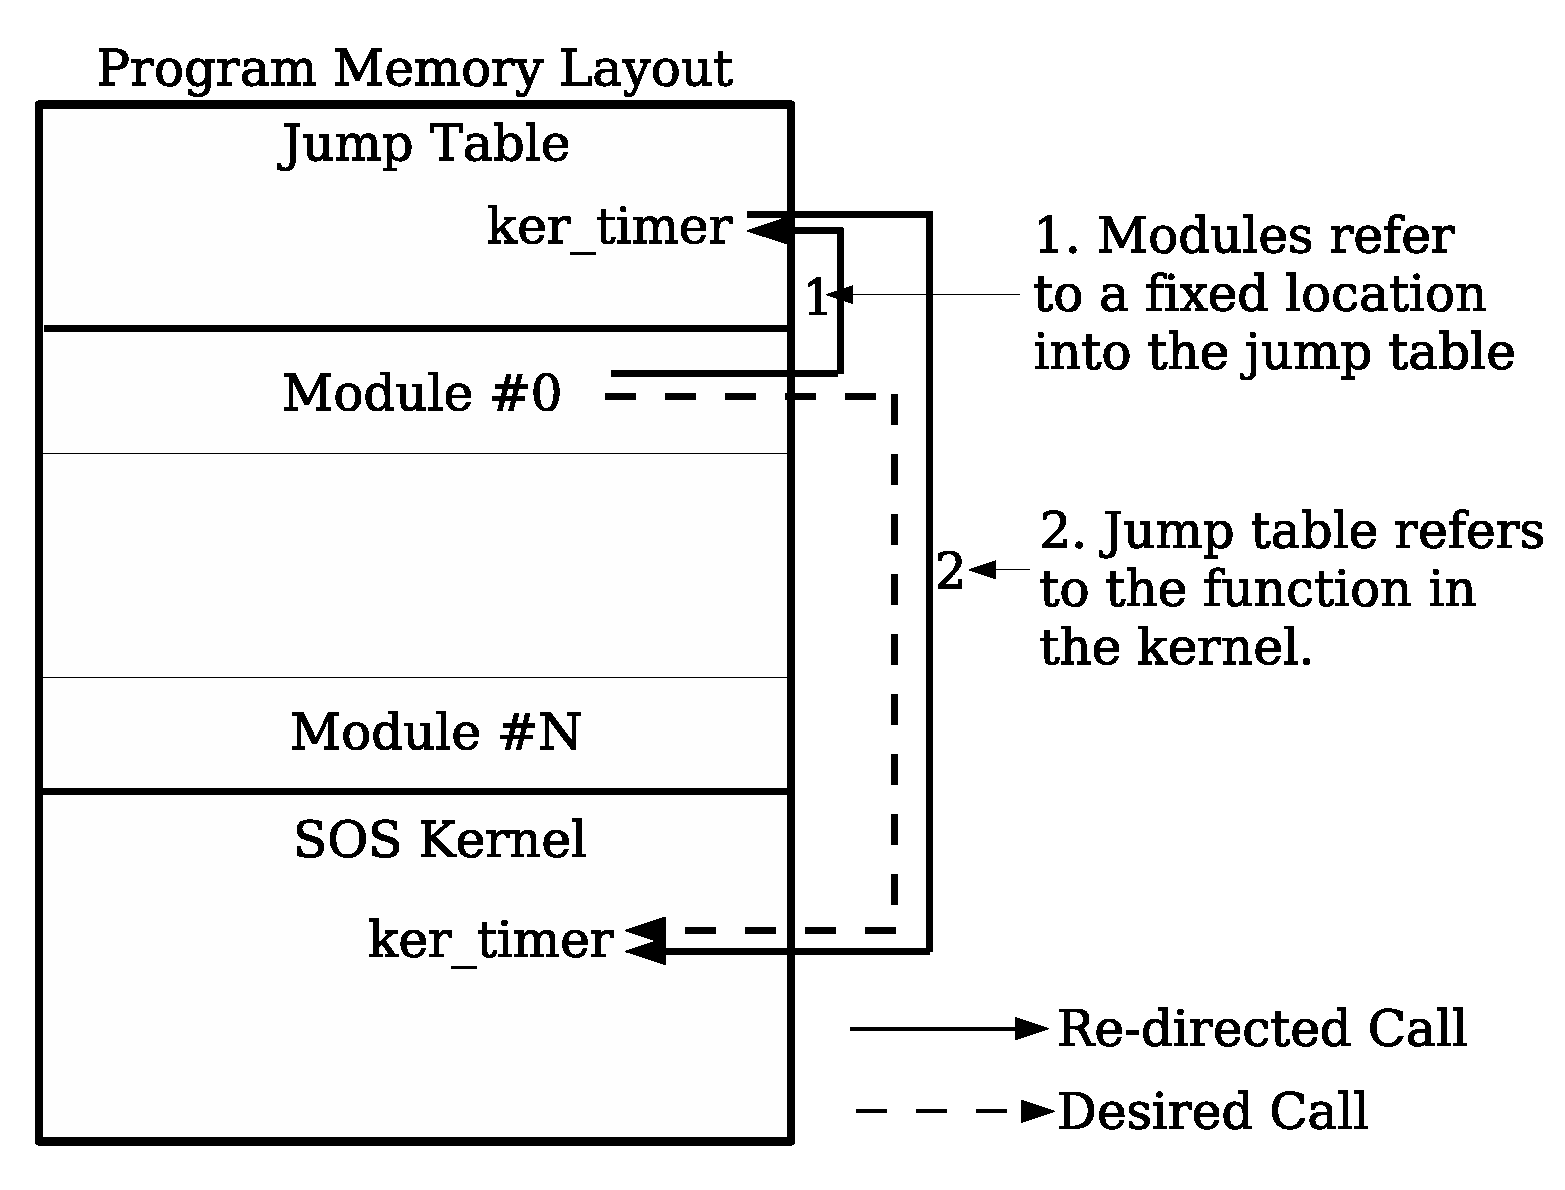
\includegraphics[width=2in,
      keepaspectratio = true]{figures/jumptable.eps}}
    \hspace{0.2in}
    \subfigure[Module
    Interactions]{\label{fig:modinteract}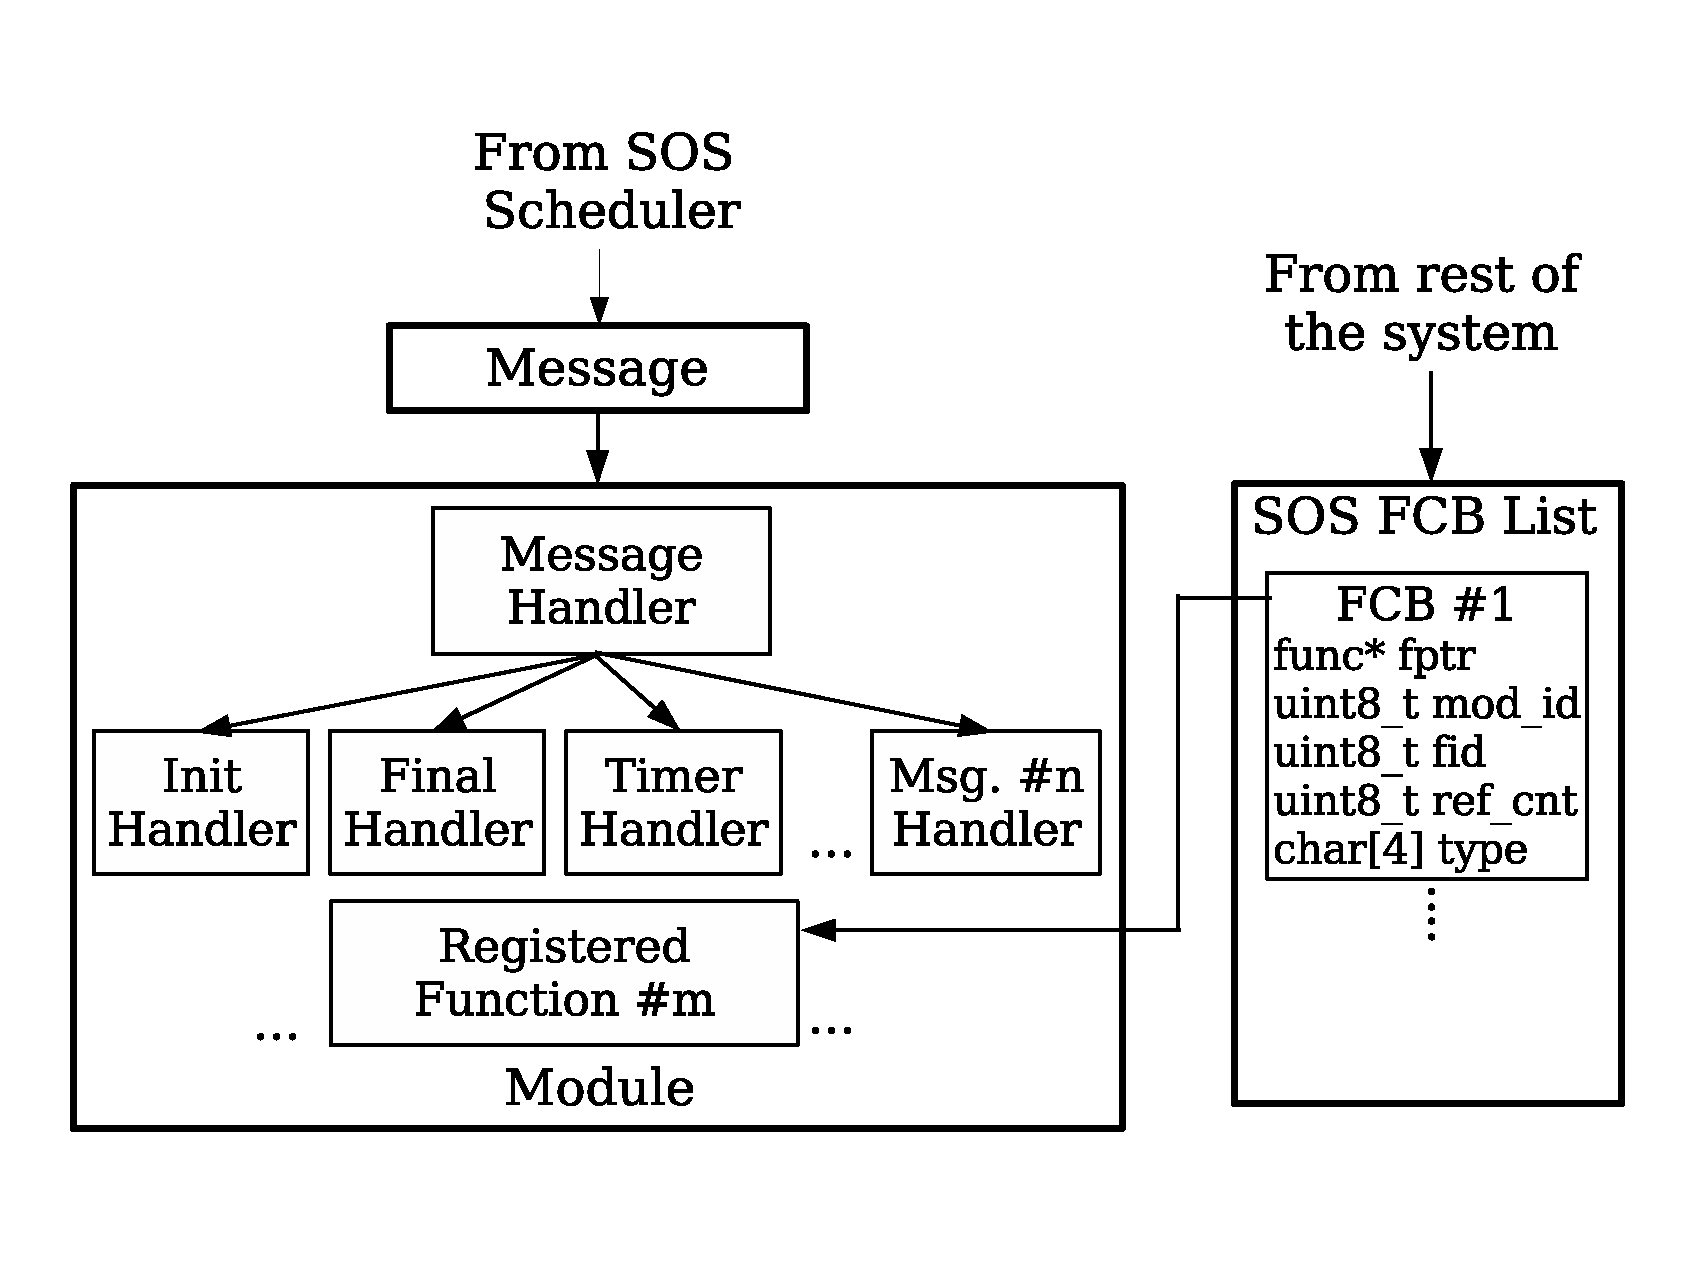
\includegraphics[width=2in,
      keepaspectratio = true]{Figures/module_interactions.eps}}
  }
  \caption{Linking SOS Module}
\end{figure}   
%
% \begin{figure}[htbp]
%   \centering
%   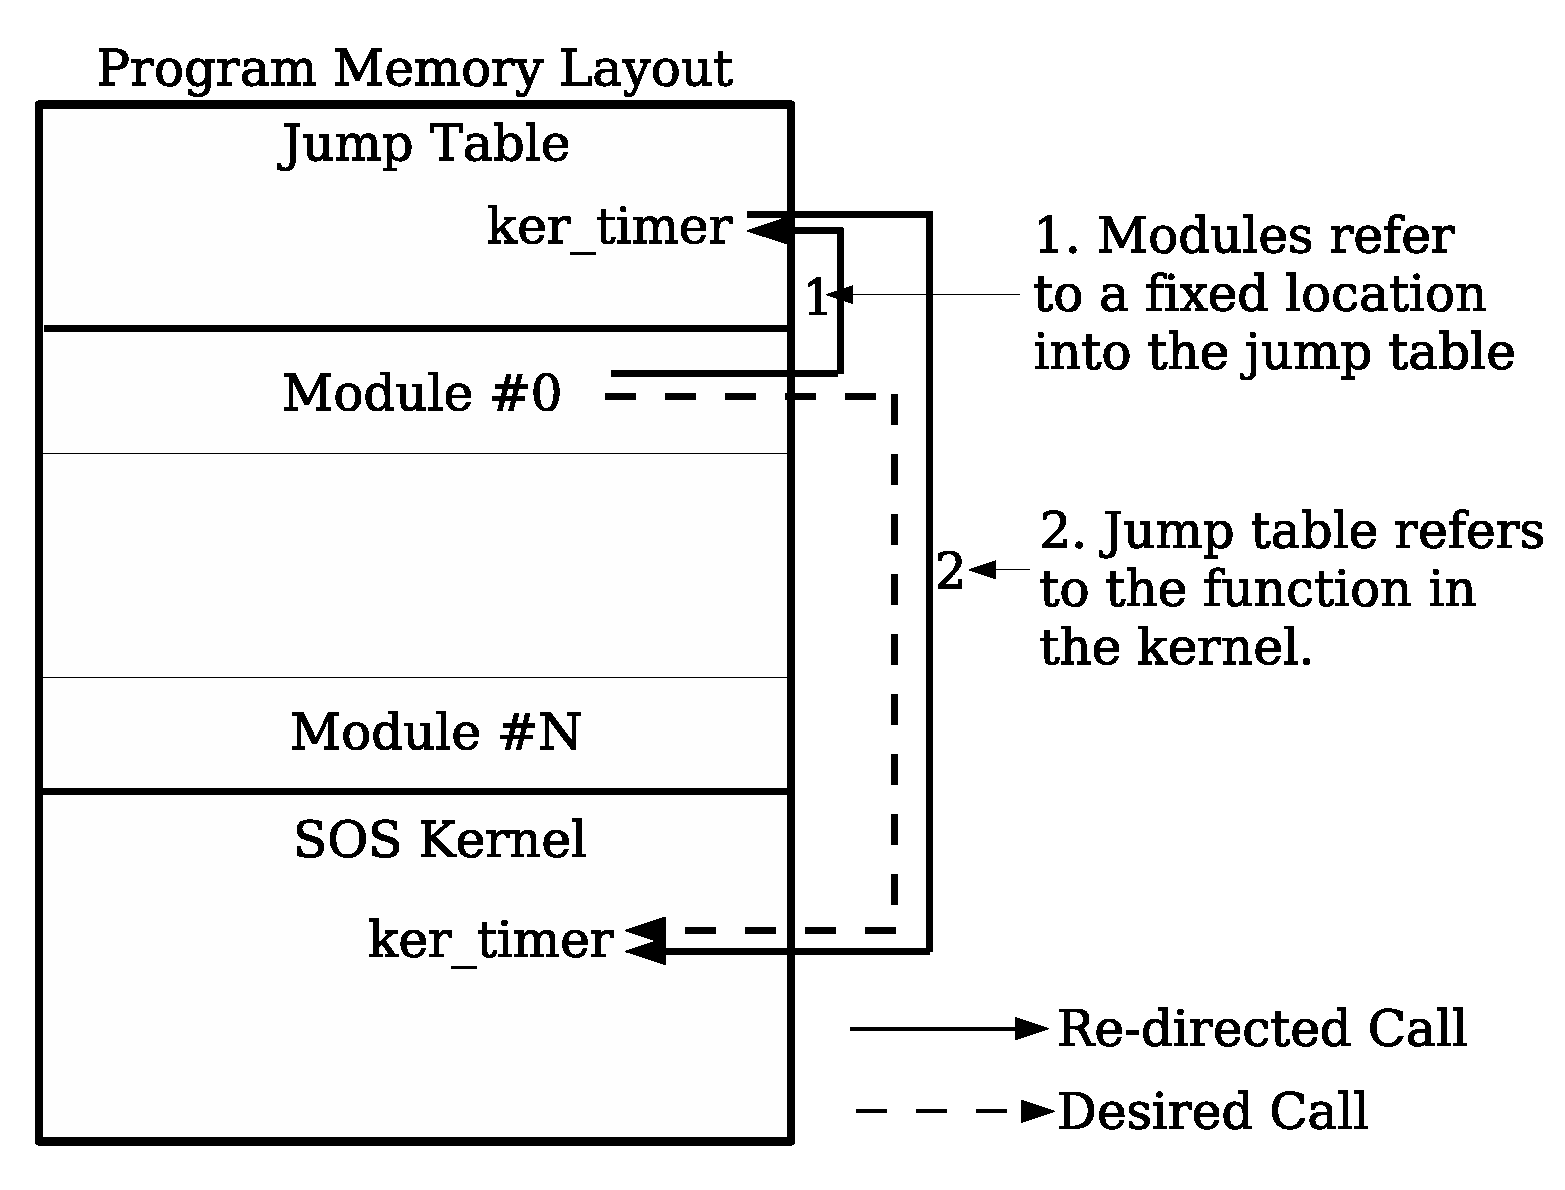
\includegraphics[height = 1.75in,
%   keepaspectratio=true]{figures/jumptable.eps} 
%   \caption{Jump Table for SOS Modules}
%   \label{fig:sosjmptbl}
% \end{figure}
%----------------------------------------------------------
\subsubsection{Message Passing}
%
The modules in SOS can communicate with other modules and the kernel
through message passing.
%
SOS modules are implemented as message handlers as shown in
Figure~\ref{fig:modinteract}.
%
The messages are annotated with the identity of the destination module
and stored in a FIFO queue within the kernel.
%
The scheduler invokes a handler function in the destination module of
a message.
%
During load time, the modules register the handler function with
the kernel.
%
%All modules are required to implement a message handler.
%
The message handlers execute in the background context.
%
The background context comprises of operations that can only be
interrupted by events occurring in the foreground context (for
e.g. hardware interrupts).
%
%A module can invoke synchronous system calls in the kernel and
%synchronous function calls in the other modules from a message
%handler.
%
After a handler terminates, the execution control is transferred back
to the scheduler.
%
SOS requires cooperative scheduling to share the processor between
multiple executing modules.
%
%---------------------------------------------------------
\subsubsection{Dynamic Memory Allocation}
% 
The SOS kernel supports dynamic memory allocation.
% 
Dynamic memory is used to store module state and to create messages to
be dispatched to other modules. 
% 
Memory is allocated using a block-based first-fit scheme to minimize
the overhead of the allocation process.
%
The size of the block is platform dependant and is 8 bytes for Mica2
sensor node.
% 
Limited memory forces SOS kernel and user modules to share a common
allocation heap; any static partitioning would be too conservative.
% 
% The dynamic memory is shared by the SOS kernel and the modules.
% 
The kernel therefore tracks ownership of memory blocks.
% 
A block's ownership can also be transferred, allowing
% 
buffers to pass easily through various modules in the system.
% 
% 
%====================================================================== 
% \subsection{System Components}
% % 
% Harbor's four components are shown in Figure~\ref{fig:sys_overview}.
% % 
% %% We first describe overall system operation.
% % 
% The system's input consists of raw user module binaries generated by a
% cross-compiler toolchain.
% % 
% The \emph{binary rewriter} is a desktop application that statically
% analyzes these binaries for potentially unsafe operations and inserts
% run-time checks to sandbox them.
% % 
% The sandboxed binary is then distributed to a network of sensor nodes.
% % 
% A \emph{verifier} running on each node verifies that incoming binaries
% are correctly sandboxed.
% % 
% Verified binaries admitted for execution interact closely
% with Harbor's run-time components, the \emph{memory map manager} and \emph{control flow
%   manager}.
% %
% \begin{figure}[htbp]
%   \centering
%   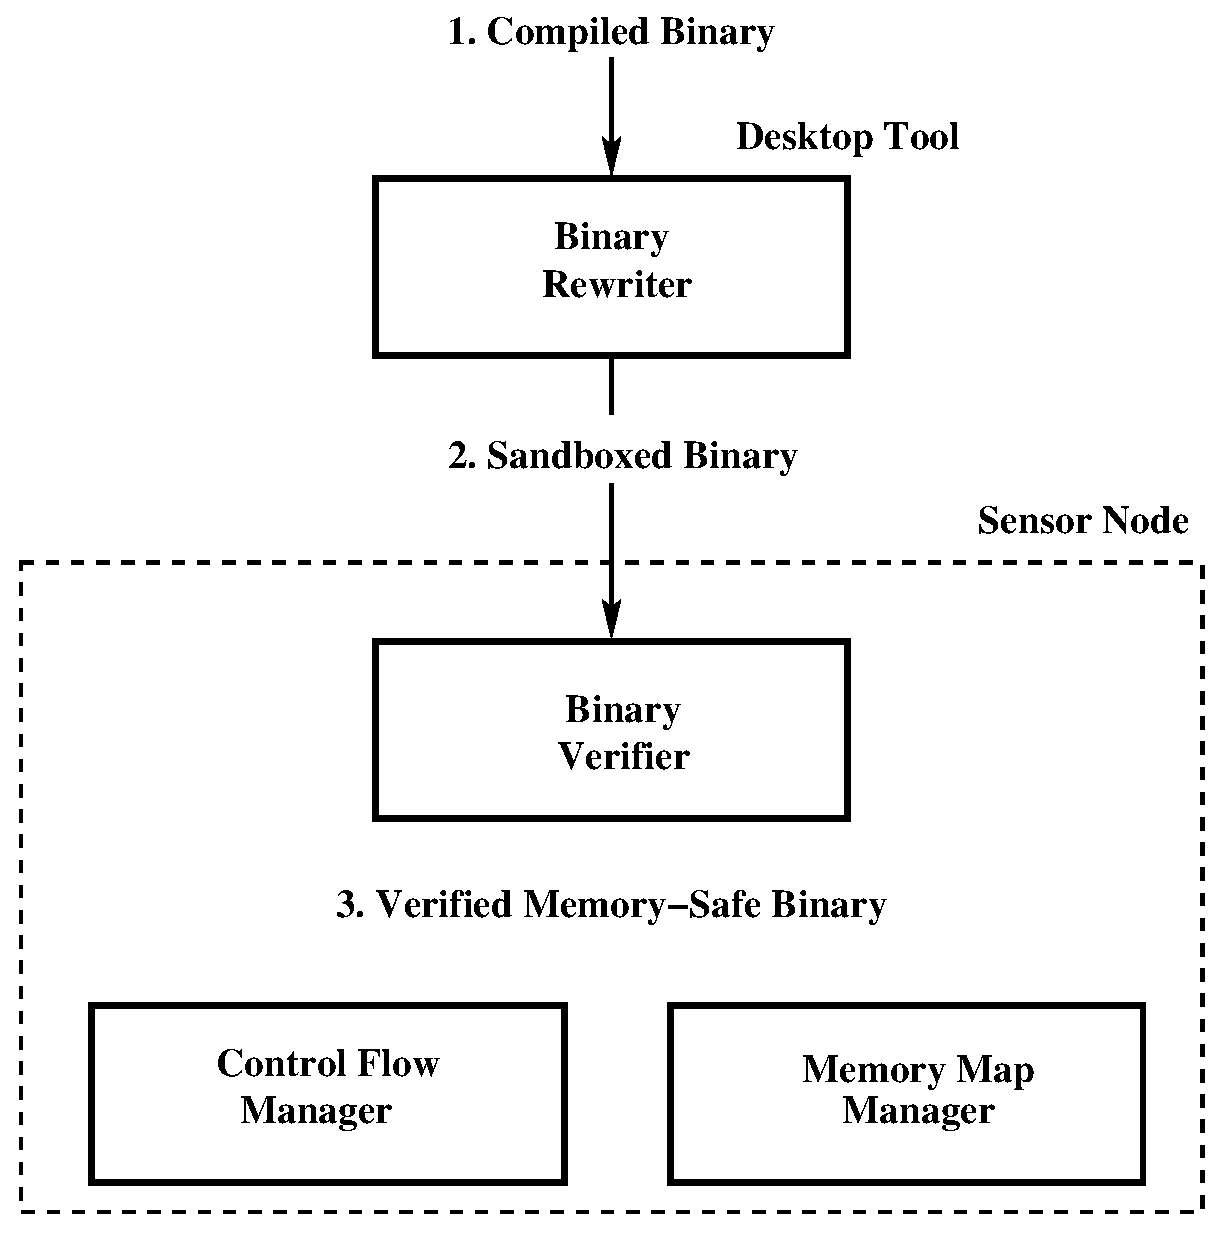
\includegraphics[height = 2.0in, keepaspectratio=true]{figures/sysoverview.eps} 
%   \caption{System Overview}
%   \label{fig:sys_overview}
% \end{figure}



%------------------------------------------------------------------
%\subsection{Summary}
%
This section positions Harbor in the category of fault isolation
techniques for
resource constrained microcontrollers.
% with limited address space.
%
Harbor isolation is more fine-grained than other approaches for sensor
networks.
%
The design of Harbor, though motivated by systems in the
desktop/server domains, introduces new techniques that address the
embedded domain's constraints.
%
Finally, the brief overview of SOS presented in this section is
essential to completely understand the implementation details.
